\documentclass[11pt, oneside]{article}   	% use "amsart" instead of "article" for AMSLaTeX format
\usepackage{geometry}                		% See geometry.pdf to learn the layout options. There are lots.
\geometry{letterpaper}                   		% ... or a4paper or a5paper or ... 
%\geometry{landscape}                		% Activate for for rotated page geometry
%\usepackage[parfill]{parskip}    		% Activate to begin paragraphs with an empty line rather than an indent
\usepackage{graphicx}				% Use pdf, png, jpg, or eps� with pdflatex; use eps in DVI mode
								% TeX will automatically convert eps --> pdf in pdflatex		
\usepackage{amssymb}
\usepackage{amsmath}
\usepackage{parskip}

\title{Ceva's Theorem}
%\author{The Author}
\date{}							% Activate to display a given date or no date

\graphicspath{{/Users/telliott_admin/Dropbox/Tex/png/}}

\begin{document}

\maketitle
%\section{}
% \subsection*{R code}
% \begin{lstlisting}  \end{lstlisting}
% \begin{center} 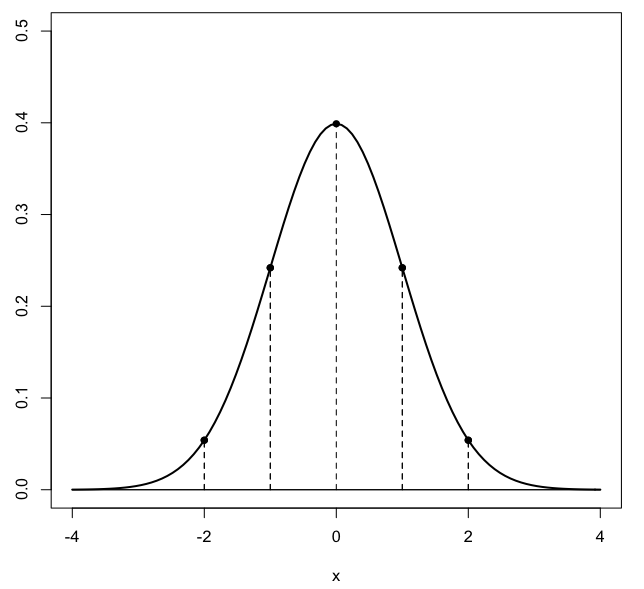
\includegraphics [scale=0.4] {gauss3.png} \end{center}
% \begin{bmatrix} a  &  b \\ c  &  d \end{bmatrix}
% \bigg |_

\Large
\noindent
We begin with the triangle shown below, picking a point $P$ to be any point inside the triangle.  Now draw line segments from each vertex through $P$ and extend them to the opposing side.
\begin{center} 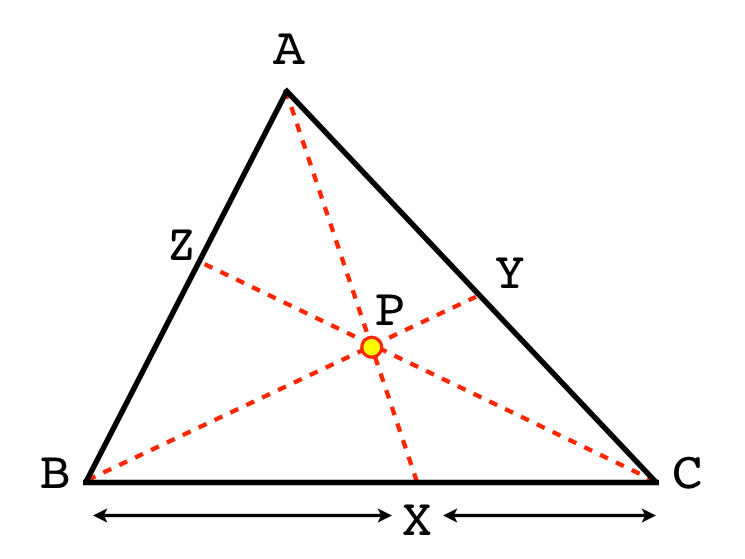
\includegraphics [scale=0.25] {ceva1.png} \end{center}
Since $P$ can be anywhere, the ratio can be anything. Let's call it $x$.
\[ BX/XC = x \]
Line $AX$ divides the whole triangle into two parts.  We know that the area of $\triangle ABX$ is in the same proportion to the area of $\triangle ACX$ as $x$, because they share the same height, while $x$ is the ratio of their bases.  Now consider the lower pair of triangles $\triangle BPX$ and $\triangle CPX$
\begin{center} 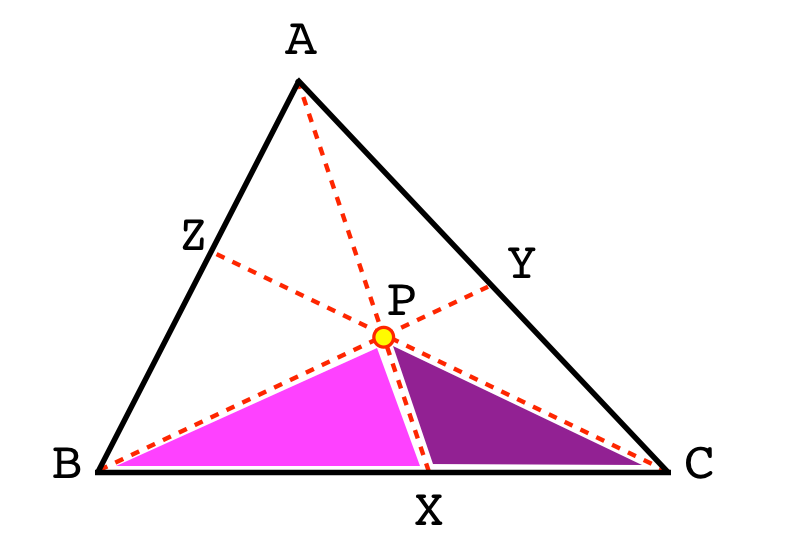
\includegraphics [scale=0.25] {ceva2.png} \end{center}
These two also have their areas in the ratio $x$, for the same reason.

The two triangles formed by the difference between these two triangles ($\triangle ABP$ and $\triangle ACP$) are shown here
\begin{center} 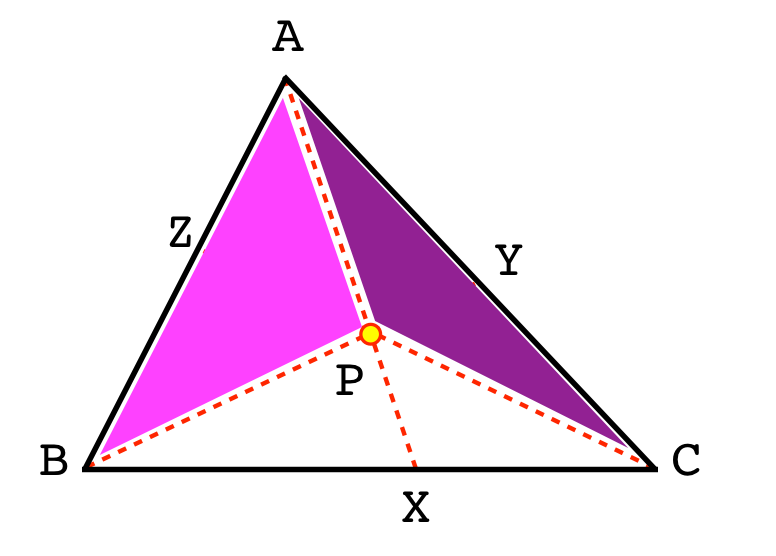
\includegraphics [scale=0.25] {ceva3.png} \end{center}
Again, the same statement is true, and for the same reason.
So, altogether, we have that
\[ \frac{|ABX|}{|ACX|} = \frac{|BPX|}{|CPX|} = \frac{|ABP|}{|ACP|} = x \]
By the same reasoning, if $y=CY/YA$
\[ \frac{|BCP|}{|ABP|} = y \]
and if $z= AZ/ZB$
\[ \frac{|ACP|}{|BCP|} = z \]
Then
\[ xyz = \frac{|ABP|}{|ACP|} \ \frac{|BCP|}{|ABP|} \ \frac{|ACP|}{|BCP|} \]
But all terms cancel, so
\[ xyz = 1 \]
And this is of course true not just for the areas but for the original line segments
\[ xyz = \frac{BX}{XC} \ \frac{CY}{YA} \ \frac{AZ}{ZB} \]
This proof also works in reverse,
\[ xyz = 1 \iff \text{3 lines cross at point P} \]
So now, for this triangle
\begin{center} 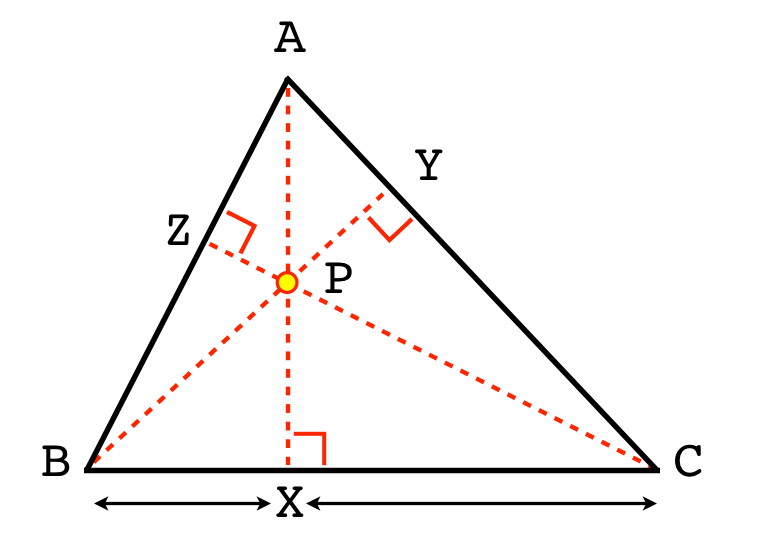
\includegraphics [scale=0.25] {ceva4.png} \end{center}
if $\alpha$ is the angle at vertex $A$ and so on, then for example,
\[ BX = AB \ cos \beta \]
and 
\[ \frac{BX}{XC} = \frac{AB \ cos \beta}{AC \ cos \gamma} \]
\[ \frac{CY}{YA} = \frac{BC \ cos \gamma}{AB \ cos \alpha} \]
\[ \frac{AZ}{ZB} = \frac{AC \ cos \alpha}{BC \ cos \beta} \]
When we construct this ratio, all the terms cancel.
\[ \frac{AB cos \beta}{AC \ cos \gamma} \ 
\frac{BC \ cos \gamma}{AB \ cos \alpha} \ 
\frac{AC \ cos \alpha}{BC \ cos \beta} = 1 \]
That means 
\[ \frac{BX}{XC} \ \frac{CY}{YA} \ \frac{AZ}{ZB} = 1 \]
Therefore, the 3 altitudes all cross at a single point.  That point is the orthocenter.

\end{document}  